% ----------------------------------------------------------
% Introdução 
% Capítulo sem numeração, mas presente no Sumário
% ----------------------------------------------------------

\chapter*[Introdução]{Introdução}
\addcontentsline{toc}{chapter}{Introdução}

Um computador moderno consiste em um emaranhado de peças que contém um ou mais processadores, alguma memória principal, alguma memória secundaria, interfaces de rede diversos periféricos como impressoras, teclado, mouse, monitor e vários outros dispositivos de entrada e saída. Podemos dizer que este é um sistema complexo, para realizar a desafiadora maratona que é compreender como cada parte funciona e gerenciar com maestria esses componentes é um grande desafio \cite{Tanenbaum2016}.
Para isso os computadores modernos são equipados com um SO esse dispositivo de software tem a função de fornecer uma plataforma simples e limpa para o usuário de forma a ajuda-lo nas entradas e saídas de dados. Em uma visão simplista podemos ver na figura~\ref{fig:figura1} onde o SO se encontra em relação entre hardware e o usuário \cite{Tanenbaum2016}. 

\begin{figure}[htpb]
    \centering
   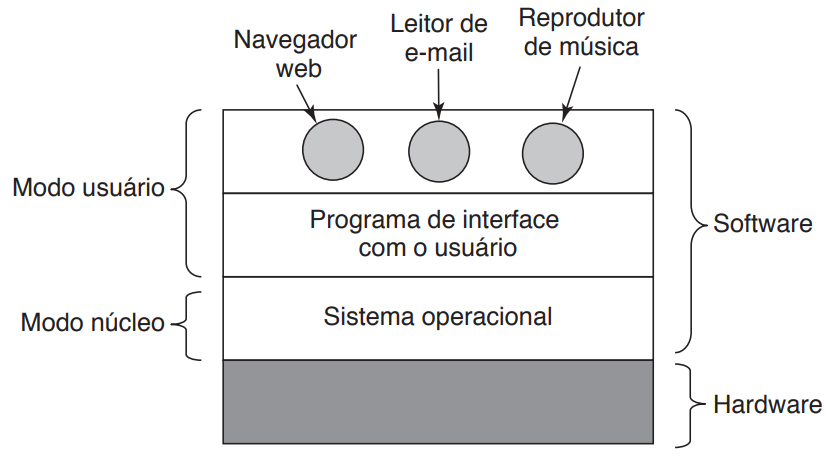
\includegraphics[scale=.4]{imagens/figura1.png}
   \caption{Onde o sistema operacional se encaixa. \cite{Tanenbaum2016}}
   \label{fig:figura1}
\end{figure}

Um sistema operacional é projetado para ocultar as particularidades de hardware (ditas "de baixo nível") e assim criar uma máquina abstrata que fornece às aplicações serviços compreensíveis ao usuário (ditas "de alto nível") \cite{Comer2012}.

%\section*{Figuras}\label{sec:figuras}
%\addcontentsline{toc}{section}{figuras}

% \section*{Tabelas}\label{sec:tabelas}
% \addcontentsline{toc}{section}{tabelas}

%\section*{Motivação}\label{sec:motivacao}
%\addcontentsline{toc}{section}{Motivação}

%\section*{Objetivos}\label{sec:objetivos}
%\addcontentsline{toc}{section}{Objetivos}


